\documentclass[12pt,a4paper,twoside]{book}


% \usepackage[utf8]{inputenc}
\usepackage[a4paper,inner=3.5cm,outer=2.5cm]{geometry}

\usepackage[titletoc,title,toc,page]{appendix}
\usepackage{tabularx}
\usepackage{array}
\usepackage{amsmath}
\usepackage{unicode-math}

\usepackage{verbatim}
\usepackage{placeins}
\usepackage{listings}
\usepackage{hyperref}
\usepackage[english]{babel}
\usepackage{tikz}
\usepackage{parskip}

\usepackage{graphicx}
\usepackage{blindtext}
\usepackage{chngcntr}
\counterwithin{table}{chapter}

\usepackage{newlfont}
\usepackage{fancyhdr}
\usepackage{indentfirst}
% \usepackage[utf8]{inputenc}
\usepackage{float}
\usepackage{hyperref}
\usepackage[capitalize,noabbrev]{cleveref}
\usepackage{soul}
\usepackage[font=footnotesize,labelfont=bf]{caption}

\usepackage{multirow}
\usepackage{hyphenat}
\hyphenation{mate-mati-ca recu-perare}

\usepackage{lscape} 

\usepackage{natbib}
\bibliographystyle{alpha}
\setcitestyle{super,open={[},close={]}}

\newcommand{\rom}[1]{\uppercase\expandafter{\romannumeral #1\relax}}

\usepackage{pdfpages}

\begin{document}
% Per spostare i vari elementi più su o più giù gioca con i valori di vspace che ci sono tra uno e l'altro
\pagestyle{empty}
\newgeometry{
    left=20mm,
    right=20mm,
    top=20mm,
    bottom=20mm
}

\begin{titlepage}

\begin{center}

% marchio di ateneo

\includegraphics[width=6.5cm,height=4.7cm]{img/marchio-di-ateneo.png}

\vspace{10mm}

% \large is 12pt
{\large{\bf{Dipartimento di Scienze ed Ingegneria Informatica}}}

\vspace{5mm}

% \Large is 14.4pt
{\Large{\bf{Corso di Informatica}}}

\vspace{15mm}

{\Huge{\bf Study of the Homomorphic Encryption }}\\
\vspace{3mm}
{\Huge{\bf Applications on Privacy Preserving }}\\
\vspace{3mm}
{\Huge{\bf Protocols}} \\

\end{center}

\vspace{10mm}

\begin{minipage}[t]{0.50\textwidth}
{\large{\bf Relatore: \\ Chiar.mo Prof.\\ FEDERICO MONTORI}}

\vspace{3mm}

{\large{\bf Correlatore: \\ Chiar.mo Prof.\\ SAVERIO GIALLORENZO}}
\end{minipage}
\hfill
\begin{minipage}[t]{0.40\textwidth}\raggedleft
{\large{\bf Presentata da: \\ DIEGO BARBIERI}}
\end{minipage}

\vspace{30mm}

\rule[0.5cm]{15.8cm}{0.6mm}

\begin{center}
{\large{\bf Sessione di Luglio 2025 \\}}
{\large{\bf Anno Accademico 2024/2025\\}}
\end{center}

\end{titlepage}

\restoregeometry
\newpage
\begin{center}
    (DA FARE ALLA FINE)\\
    5 parole chiave per caratterizzare il contenuto della dissertazione:\\ (se non ti piacciono così sparse puoi anche semplicemente scriverle su una riga sola)
\end{center}

% https://tex.stackexchange.com/questions/26538/words-scattered-randomly-in-on-coverpage
\begin{tikzpicture}[overlay,remember picture,shift=(current page.center)]
\pgfmathsetseed{3}


\foreach [count=\count] \word in {Parola 1, parola 2, parola 3, parola 4, parola 5} {
\node [
    xshift={(mod(\count,3)-1)*(\paperwidth/4)},
    yshift={(mod(\count,7)-3)*(\paperwidth/6)},
    xshift=rand*4cm,
    yshift=rand*2cm,
    % rotate=rand*35,
    % opacity=rnd*0.5+0.125,
    font=\large] {\word};
}
\end{tikzpicture}
\newpage

\topmargin=6.5cm
\begin{flushright}
\emph{
\LARGE{La dedica}\\\vspace{2mm}
\LARGE{anche quella se vuoi}\\\vspace{3mm} 
\LARGE{su più righe} 
}
\end{flushright}
\newpage~\newpage
\pagenumbering{gobble}

\newgeometry{
    left=20mm,
    right=20mm,
    top=20mm,
    bottom=20mm
}


\chapter*{Abstract}
Abstract qui (ti consiglio di farlo alla fine)

\topmargin=-1cm
\tableofcontents
\thispagestyle{empty}
\listoftables
\thispagestyle{empty}
\listoffigures
\thispagestyle{empty}
\newpage~\newpage

\pagenumbering{arabic}
\setcounter{chapter}{-1}
\raggedbottom
\chapter{Introduction} \label{chap:intro}

\pagestyle{plain}
\setcounter{page}{1}


\chapter{Background}
\section{Request-Response Protocol}
The Request-Response protocol is a fundamental communication pattern in distributed systems where a client sends a request to a server and waits for a response. This synchronous communication model is characterized by its simplicity and direct interaction between parties, making it suitable for operations requiring immediate feedback and confirmation.

\subsection{HTTP}
HTTP (Hypertext Transfer Protocol) is the foundation of data communication on the World Wide Web. It operates as a request-response protocol, allowing clients to request resources from servers and receive responses. HTTP supports various methods (GET, POST, PUT, DELETE) for different types of operations and is extensible through headers and status codes.

\subsubsection{HTTPS}
HTTPS is a version of HTTP built on the SSL/TLS protocol, providing secure communication over a computer network. It encrypts data exchanged between clients and servers, ensuring confidentiality and integrity. HTTPS is essential for protecting sensitive information from eavesdropping and tampering.

One of the key features of HTTPS is its use of certificates to authenticate the server, ensuring that clients are communicating with the intended entity. This is possible through a relatively high usage of computational resources, which is a trade-off for the enhanced security it provides.

\subsection{Reuqest-Response in IoT devices}
HTTPS is a commonly used choice also for IoT devices. However, its usability is often limited due to a number of factors:
\begin{itemize}
    \item \textbf{Resource Constraints\cite{mazhar2023iotsecurity}}: Encrypting and decrypting certificates standards (RSA, EEC, AES) can be computationally expensive, which is a significant concern for IoT devices with limited processing power and memory.
    \item \textbf{Lack of Secure Firmware Updates\cite{cyberark2024iot}}: Many IoT devices do not support secure firmware updates, making it difficult to patch vulnerabilities in the HTTPS implementation.
    \item \textbf{Weak or Nonexistent Certificate Validation\cite{bishopfox2020weakcertificates}}: Many IoT devices do not validate server certificates properly, leading to potential vulnerabilities.
\end{itemize}

\section{Publish-Subscribe Protocol}
The Publish-Subscribe (Pub/Sub) protocol is an asynchronous messaging pattern where senders (publishers) categorize messages into topics without knowledge of the receivers (subscribers). Subscribers express interest in specific topics and receive messages published to those topics. This decoupled architecture enables scalable and flexible communication in distributed systems.

\subsection{MQTT}
MQTT (Message Queuing Telemetry Transport) is a lightweight, open-source messaging protocol designed for constrained devices and low-bandwidth, high-latency networks. It implements the publish-subscribe pattern over TCP/IP, providing three quality of service levels for message delivery and supporting various security features.

The protocol defines three main network entities:
\begin{itemize}
    \item \textbf{Message Broker}: The central component that manages message routing between publishers and subscribers. It receives messages from publishers and forwards them to subscribers based on their subscriptions.
    \item \textbf{Publisher}: A client that sends messages to the broker on specific topics. 
    \item \textbf{Subscriber}: A client that expresses interest in specific topics and receives messages published to those topics by the broker.
\end{itemize}

\subsubsection{MQTT Quality of Service Levels}

MQTT provides three quality of service (QoS) levels to ensure message delivery reliability:
\begin{itemize}
    \item \textbf{QoS 0 (At most once)}: The message is delivered at most once, with no acknowledgment from the receiver. This level is suitable for applications where occasional message loss is acceptable.
    \item \textbf{QoS 1 (At least once)}: The message is guaranteed to be delivered at least once, with acknowledgment from the receiver. This level ensures that messages are not lost but may result in duplicates.
    \item \textbf{QoS 2 (Exactly once)}: The message is guaranteed to be delivered exactly once, using a four-step handshake process. This level provides the highest reliability but incurs more overhead.
\end{itemize}

\subsubsection{MQTT Security}

As we mentioned, one of the key features of MQTT is the possibility to scale the protocol to fit the needs of the application. This is possible by using different security features, such as TLS/SSL for secure communication, authentication mechanisms to verify client identities, and access control lists to restrict topic access. These features help protect against unauthorized access and ensure the integrity of messages exchanged between clients.

\subsubsection{MQTT Workflow}

\begin{figure}[h]
    \centering
    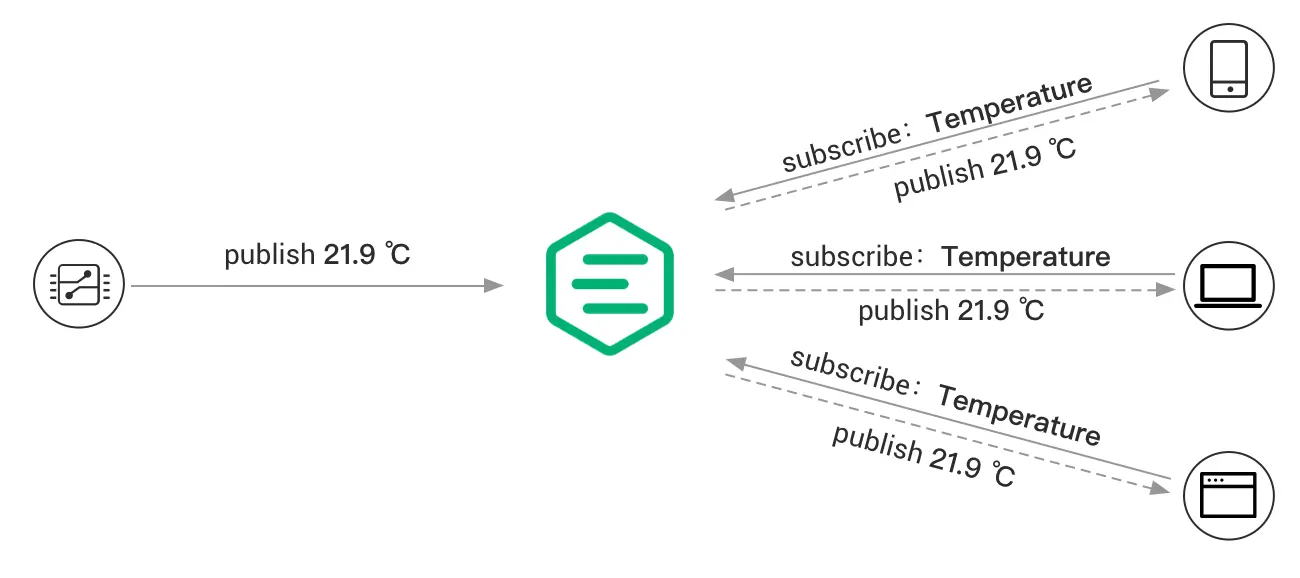
\includegraphics[width=10.5cm,height=4.7cm]{img/mqtt-workflow-example.png}
    \caption{MQTT Workflow}
    \label{fig:mqtt-workflow}
\end{figure}

Generally, the MQTT workflow starts with the client establishing a connection to the broker, using a TCP/IP connection with optional TSL/SSL security. Once connected, the client can publish messages to specific topics or subscribe to topics of interest. The broker then routes messages to subscribers based on their subscriptions.

\subsection{LA-MQTT} \label{sec:la-mqtt}
LA-MQTT (Location-Aware MQTT) extends the standard MQTT protocol by incorporating location-based features. It enables spatial queries and location-aware message routing, making it particularly suitable for IoT applications requiring geographical context in message distribution.

The protocol is first intruduced with the purpose of resolving the limitations of traditional MQTT in handling location-based data\cite{montori2022lamqtt}.

\begin{table}[h]
\small
\begin{tabularx}{\linewidth}{|l|X|X|X|p{4cm}|}
\hline
\textbf{API} & \textbf{Subject} & \textbf{MQTT OP} & \textbf{Topic} & \textbf{Payload} \\ \hline
Position publish & MC & Publish & GPS\_DATA & $\{position: ( P_i )\}$ \\ \hline
Topic subscription & MC & Subscribe & $C(i, t_s)$ & * \\ \cline{2-5}
 & MC & Publish & MC\_SUB & $\{ mc: i, topic: t_s \}$ \\ \hline
Geofence publish & LDS & Publish & GEOFENCE\_DATA & $\{topic: t_s, content: c_s, $\newline$region: g_s, event: e_s\}$ \\ \hline
Content publish & Backend & Publish & $C(i, t_s)$ & $\{content: c_s\}$ \\ \hline
\end{tabularx}
\caption{The LA-MQTT Publish-subscribe Operations}
\label{table:la-mqtt}
\end{table}

The table \ref{table:la-mqtt} summarizes the main operations of the LA-MQTT protocol, highlighting the interactions between clients (MC), location data sources (LDS), and the backend system.

Those operations include:
\begin{itemize}
    \item \textbf{Position Publish}: MC publish their GPS data to the broker, allowing other clients to receive updates on their positions.
    \item \textbf{Topic Subscription}: MCs subscribe to specific topics, enabling them to receive messages related to their areas of interest.
    \item \textbf{Geofence Publish}: LDSs publish geofence data, which includes the topic, content, region, and event associated with the geofence.
    \item \textbf{Content Publish}: The backend publishes content related to the subscribed topics, forwarding it to the subscribed MCs.
\end{itemize}

\section{Universal Location Referencing}
Universal Location Referencing provides standardized methods for encoding and representing geographical locations. These systems ensure consistent and unambiguous location representation across different applications and platforms.

\subsection{Cantor Pairing}

Cantor Pairing is a mathematical technique that uniquely maps two natural numbers to a single natural number. This bijective function $\pi: \mathbb{N} \to \mathbb{N}$ is particularly useful in computer science for combining two coordinates into a single value while maintaining the ability to recover the original coordinates.

More formally, the Cantor pairing function is defined as:
\[
    \pi(x, y) = \frac{(x + y)(x + y + 1)}{2} + y
\]

Although this function does not preserver algebraic properties, it porvides some unique properties derived from the fact that it is segmenting the two-dimansional space into a zig-zag pattern.

\[
    \pi(x, y) + 1 = \pi(x - 1, y + 1)
\]

Moreover, we also need to define the bheavior of the function when hits the boundaries of the first quadrant:

\[
    \pi(x, 0) + 1 = \pi(x + 1, 0)
\]

At last we denote the starting point of the Cantor pairing function as \( \pi(0, 0) = 0 \). This means that the function starts at the origin of the two-dimensional space and maps it to zero in the one-dimensional space. The inverse of the Cantor pairing function can be computed as follows:
\[
    \pi^{-1}(z) = \left( \frac{n(n + 1)}{2} - z, z - \frac{n(n + 1)}{2} \right)
\]
Where \( n \) is the largest integer such that \( \frac{n(n + 1)}{2} \leq z \). This allows us to retrieve the original coordinates \( (x, y) \) from the single value \( z \).

This function is widely used in computer science, particularly in data structures and algorithms, where it is necessary to map multi-dimensional data to a single dimension for efficient storage and retrieval. It is also used in various applications such as database indexing, spatial data representation, and cryptography.


\vspace{5mm}

\begin{figure}[h]
    \centering
    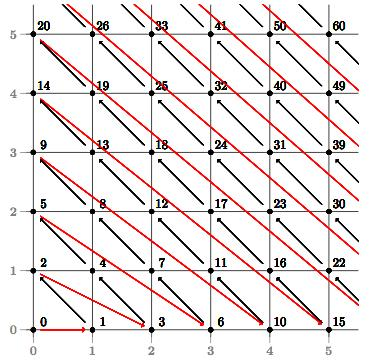
\includegraphics[width=6.5cm,height=4.7cm]{img/cantor-pairing.jpg}
    \caption{Visualization of the Cantor pairing function mapping two-dimensional coordinates to a single value}
    \label{fig:cantor}
\end{figure}

\vspace{5mm}

\section{Space Filling Curves}
Space Filling Curves are mathematical curves that pass through every point in a multi-dimensional space. They provide a way to map multi-dimensional data to a single dimension while preserving spatial locality, making them valuable for spatial indexing and data organization.

The most common space-filling curves include:
\begin{itemize}
    \item \textbf{Z-order Curve}
    \item \textbf{Hilbert Curve}
\end{itemize}

%\vspace{5mm}

\begin{figure}[h]
    \centering
    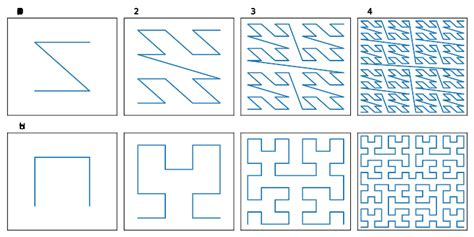
\includegraphics[width=6.5cm,height=4.7cm]{img/hilbert-z-order.jpg}
    \caption{Comparison of Z-order and Hilbert curves in two-dimensional space}
    \label{fig:space-filling}
\end{figure}

\vspace{5mm}

The Hilbert Curve is particularly notable for its ability to preserve locality, meaning that points that are close in multi-dimensional space remain close in the one-dimensional representation.

On the other hand, the Z-order Curve, preserve the order of positions in a grid-like manner, making it suitable for applications requiring efficient spatial queries. Thus, it's possible to reduce the problem of finding matching points into finding the maximum prefix of two bit strings.

\subsection{Z-order Curve}
As mentioned, the Z-order curve is one of the most widely used space-filling curves. It maps multi-dimensional data into a single dimension, similar to the Cantor encoding function. Conversly, it has some some useful properties, when applied to spacial data, such as preserving locality and allowing efficient range queries.

\subsubsection{Z-order Encoding}

The encoding process for Z-order involves interleaving the bits of the coordinates of a point in a multi-dimensional space. For example, given a point with coordinates \( (x, y) \), the Z-order encoding can be represented as:
\[
    Z(x, y) = \sum_{i=0}^{n} (x_i \cdot 2^{2i} + y_i \cdot 2^{2i+1})
\]

Where:
\begin{itemize}
    \item \( x_i \) and \( y_i \) are the bits of the binary representation of the coordinates \( x \) and \( y \).
    \item \( n \) is the number of bits used to represent each coordinate.
\end{itemize}

\subsubsection{Z-order Decoding}
The decoding process retrieves the original coordinates from the Z-order encoded value. Given a Z-order value \( Z \), the decoding can be performed by extracting the bits corresponding to each coordinate:
\[
    x = \sum_{i=0}^{n} (Z \pmod{ 2^{2i+2} }) \cdot 2^i
\]
Where:
\begin{itemize}
    \item \( Z \pmod{ 2^{2i+2} } \) extracts the bits corresponding to the \( i \)-th coordinate.
    \item The result is then shifted and combined to reconstruct the original coordinate \( x \).
\end{itemize}

\subsubsection{Z-order Querying}
Let's consider a scenario where we want to find all points within a specific range in a two-dimensional space. We define \( P \) as the set of points in the space, and we want to find all points \( p \in P \) such that:
\[
    p.x \in [x_{min}, x_{max}] \quad \text{and} \quad p.y \in [y_{min}, y_{max}]
\]

We can leverage the Z-order encoding to efficiently query this range. This is possible by calculating the order of the encoding that we want to find. 
By definition we can represent the GPS coordinates of a point \( (x_p, y_p) \) into a point \( e_p \). This point will be represented in the space of \( n \) orders, each contained in \( \mathbb{Z}_4 \).

\subsubsection{Maximum Common Prefix Search}
A key operation in Z-order based spatial queries is finding the maximum common prefix between two Z-order encoded values. This operation is fundamental for determinating spatial relationships between points.

Given two Z-order encoded values \( Z_1 \) and \( Z_2 \), we can find the maximum common prefix by following three steps. Firstly, we convert both values to their binary representation. Then, we compare the bits from left to right, stopping at the first position where the bits differ. Finally, we extract the common prefix up to that point. The cited algorithm shows that in the worst case, the maximum common prefix can be found in \( O(n) \) time, where \( n \) is the number of bits in the Z-order encoding.

The length of the common prefix determines the size of the smallest bounding box that contains both points. This property is particularly useful for:
\begin{itemize}
    \item Finding the smallest region containing multiple points
    \item Determining if points are within a certain distance of each other
    \item Optimizing spatial range queries
\end{itemize}

For example, consider two points with Z-order encodings:
\begin{align*}
    Z_1 &= 3310_4 \\
    Z_2 &= 3312_4
\end{align*}
The maximum common prefix is \( 331_4 \), indicating that these points share the same region in the first three orders of the encoded space. We used base 4 because it's the easiest way to visualize which of the four quadrants the point belongs to, as each digit represents a quadrant in a two-dimensional space.

This prefix-based approach can be extended to handle range queries by:
\begin{enumerate}
    \item Encoding the query range boundaries
    \item Finding the maximum common prefix of the range
    \item Generating all possible Z-order values that share this prefix
\end{enumerate}

The efficiency of this approach comes from the fact that we can perform these operations using simple bitwise operations, making it suitable for real-time applications.


\section{Privacy Preserving}
Privacy Preserving techniques ensure the protection of sensitive information while allowing necessary computations and data processing. These methods are crucial in maintaining confidentiality in distributed systems and data analysis. For example, in the context of location-based services, privacy-preserving techniques allow for the sharing of location data without revealing exact coordinates, thus protecting user privacy.

\subsection{Homomorphic Encryption}
Homomorphic Encryption(HE) is a form of encryption that allows specific types of computations to be performed on ciphertext, producing an encrypted result that, when decrypted, matches the result of operations performed on the plaintext.

Let's denote \( \xi_k \) as the encryption function, \( \xi_k^{-1} \) as the decryption function, and \( f \) as a function that can be computed on plaintexts. Homomorphic Encryption satisfies the property:
\[
    \xi_k(f(x)) = f(\xi_k(x))
\]

During the years, several Homomorphic Encryption schemes have been proposed, each with different properties and capabilities. The scheme used druing our tests is the Brakerski-Gentry-Vaikuntanathan (BGV, 2011) scheme \cite{Brakerski2012-wj}, which is a leveled fully homomorphic encryption scheme that supports both addition and multiplication operations on encrypted data. The BGV scheme is particularly notable for its efficiency and ability to handle large integers, making it suitable for practical applications in privacy-preserving computations.
This scheme was based on the security of \textbf{(Ring) Learning With Errors} (RLWE) \crer{subsec:rlwe) problem, which is a hard problem in lattice-based cryptography. The need for such a scheme arises from the increasing demand for secure computations in various fields, including cloud computing, data analysis, and machine learning. This type of new technology is designed to resist quantum computer and cryptanalysis. 

\subsubsection{Security foundation: (Ring) Learning With Errors (RLWE)} \label{subsec:rlwe}

The security of lattice-based FHE schemes, especially BGV, rests on the hardness of the Ring Learning With Errors (RLWE) problem, a ring-based variant of the Learning With Errors (LWE) problem introduced by Lyubashevsky, Peikert, and Regev in 2010 \cite{Lyubashevsky2010-jo}.
. In RLWE, one works over a polynomial ring modulo both a prime $q$ and an irreducible polynomial $f(x)$:

\[
    a(x) = a_0 + a_1 x + \ldots + a_{n-1} x^{n-1}, \text{where } a_i \in \mathbb{Z}_q
\]

Samples are of the form $(a(x),\,b(x)=a(x)s(x)+e(x))$, where $e(x)$ is a small “error” polynomial. Recovering $s(x)$ given many such samples is presumed hard, based on reductions to the Shortest Vector Problem (SVP) in ideal lattices.

\subsubsection{Homomorphic Encryption Types}

\textbf{Fully Homomorphic Encryption (FHE)} allows the evaluation of arbitrary circuits of additions and multiplications over encrypted data, without decryption. However, earlier FHE schemes suffered from inefficiencies, particularly due to large growth of noise. The BGV scheme answered these challenges by avoiding Gentry’s “bootstrapping” \cite{brakerski2011leveled} step via \emph{leveled} evaluation, and controlling noise through \emph{modulus switching} and \emph{relinearization} techniques.

\textbf{Partially Homomorphic Encryption (PHE)} supports only one type of operation—either addition (e.g., Paillier) or multiplication (e.g., RSA variants). These are faster than FHE but limited in expressiveness, making them suitable for simpler tasks where only one operation type is required.

\section{Usage of HE for Matching}
Homomorphic Encryption can be used to securely match location. To archive this, we can use different techniques such as:
\begin{itemize}
    \item \textbf{Distance Calculation}: It is archived by tweeking the distance calculation algorithms (e.g., Euclidean distance, Cosine similarity, Manhattan Distance) to work with encrypted coordinates. The main limit comes with the constraint that the operations must be compatible with the encryption scheme used. For instance, calculating the squared Euclidean distance between two points \( (x_1, y_1) \) and \( (x_2, y_2) \) can be expressed as:
    \[
        d^2 = (x_1 - x_2)^2 + (y_1 - y_2)^2
    \]
    That can be computed homomorphically, and then decrypted before computing the square root to get the actual distance.
    \item \textbf{Encoding Coordinates}: By encoding coordinates into a grid-like structure, we can reduce the problem into finding two different points sharing the same area-encoding. This apporach comes with some limitations, mainly related to the precision of the approximation and the size of the grid. Still, it allows for efficient matching of points within a specific area without revealing their exact coordinates.
\end{itemize}

\subsubsection{Privacy-Preserving Z-order Queries}
When implementing privacy-preserving location queries using Z-order encoding, we can employ homomorphic encryption to protect sensitive location data \cite{zhang2020privacy}. Let's consider a scenario where a user \( A \) wants to share their location with user \( B \) while maintaining privacy:

\begin{itemize}
    \item Let \( QK_A \) be the QuadKey representation of \( A \)'s location
    \item Let \( M_B \) be the bit mask specified by \( A \) for user \( B \)
    \item The service provider (SP) performs homomorphic multiplication: \( QK_A \otimes M_B \)
\end{itemize}

To ensure unambiguous results, we increment each value in \( qk_i \in QK_A \) by one before encryption, such that \( qk_i \in \{1,2,3,4\} \). In this scheme \cite{zhang2020privacy}:
\begin{itemize}
    \item A bit mask value of 1 preserves the location data
    \item A bit mask value of 0 masks the location data
\end{itemize}

After decryption on the client device, we:
\begin{enumerate}
    \item Remove any zero values
    \item Convert the elements back to \( \mathbb{Z}_4 \)
    \item Generate a masked QuadKey string that produces a bounding box with the desired level of detail
\end{enumerate}

This approach is computationally efficient as it requires only one round of homomorphic multiplication. The resulting bounding box effectively hides both precise locations and movement patterns, providing privacy even against colluding users.

For example, given a precise GPS coordinate \( (43.084451, -77.680069) \), the system can generate bounding boxes of varying sizes based on the privacy preferences (where \( d \) represents the level of detail). This ensures that location data is shared at an appropriate granularity while maintaining user privacy.

% TODO: add other type of queries

\subsection{PHE and FHE Implications}
The choice between Partially and Fully Homomorphic Encryption has significant implications for system performance, security, and functionality. As previously discussed, the two methods used for proximity checks in a location-based scenario require careful consideration of the encryption scheme.

If the requirements only involve checking whether two positions share a common area, leveraging the speed and simplicity of the Z-order approach is recommended. Conversely, if the goal is to compute a precise floating-point distance value, a homomorphically encrypted distance function (e.g., Euclidean distance) may be necessary. However, it is important to note that in this case, the final result may be affected by computational noise inherent to FHE operations.


\chapter{System Architecture}
In this chapter, we present the system architecture for the proposed privacy-preserving location matching protocol. The main idea is to apply the principles of homomorphic encryption to location-based services, allowing clients to securely publish and performing queries using their positions without revealing sensitive information.

\section{Use Case}
To clearly understand the system operations, let's first analyze the use case of a client that wants to find the closest parking spot available. The client needs to compute the distances between its position and the parking spots, and finally decide whether to park or not and where.

Even through it seems a simple and straightforward mechanism, if we want to move the operations to the server, in order to preserve computational resources on the client side, a lot of challenges arise. The first one is to securely share the position of the client with the server, without exposing it to the workers. The second one is is not to leak sensible information about the clients, after the computation is finished.

In this scenario, it's not enough to simply encrypt the positions of the clients, as the workers need to compute the distances between the positions of the clients and the parking spots, that are also encrypted with a different key. To resolve this problem, we could just leave the parking position in clear text on the database, but this would expose the parking spots to the workers, that could then leak the information for profit. Thus, by selling the parking spots to third parties, they could are compromising the privacy of the system. In order to avoid this, and also achieve a full privacy-oriented protocol, we need to use a re-encryption mechanism, that allows the workers to compute the distances between the positions of the clients and the parking spots, without revealing the positions of the clients to the workers.

The distance problem is avoided by using the Z-order encoding, that allows us to reduce the problem of finding matching points into finding the maximum prefix of two bit strings. In our use case, the simulated server will perform a simple encrypted subtraction between the positions of the clients and the parking spots. At last, the only the client will be able to decrypt the result, which is a simple integer value that represents the distance between the two points (If the value is 0 is a perfect match). The client can then use this value to decide whether to park or not, and where. 

\section{System Overview}
The protocol is designed to combine a standard request-response protocol with a publish-subscribe mechanism.


\begin{figure}[h]
    \centering
    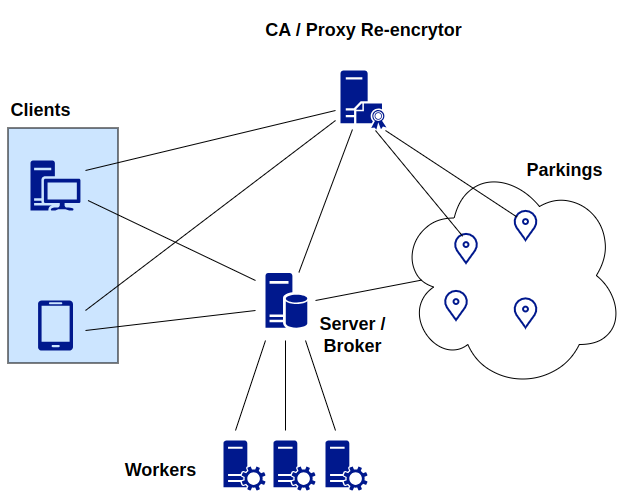
\includegraphics[width=8.5cm,height=5.5cm]{img/architecture-scheme.png}
    \caption{Visualization of the system architecture for the proposed privacy-preserving location matching protocol.}
    \label{fig:architecture}
\end{figure}

Homomorphic encryption incurs high computational costs, so the system optimizes performance by splitting the workload: the server handles only essential data processing, while workers compute the distances between client positions. Since HE allows computations on encrypted data, this approach preserves the privacy of clients' locations without compromising efficiency.

\section{Actors}

\subsection{Location Data Source}
The Location Data Source (LDS), commonly referred to as sensors or parkings, are responsible for collecting and publishing location data. In our system, we assume they independently publish their data to the broker, based on the event they register. For instance, if a sensor detects a free parking spot, it publishes the information to the broker, that will start the encryption protocol. This happens also when a parking spot is occupied, allowing the system to keep track of the available parking spots in real-time.

Note that by maintaining the availability of the parking spots, independent from the clients, we can ensure that the system is able to provide privacy-preserving updates to the server. Conversely, if the clients were also responsible for reserving the parking spots, they would need to expose their positions to the server, which would compromise the privacy of the system.

\subsection{Mobile Clients}
MCs or Mobile Clients are the users of the system. Their main interest is to receive updates on the closest available parking spots, based on their current position. 

In our system, the client's responsibilities are very limited, as they do not trust the server and all the other actors involved in the protocol. They only need to publish their encrypted position to the server, wait for the computation to finish, and then receive the results.

\subsection{Server}
The Backend Server (commonly called Information Broker) is the central component of the system, responsible for managing the communication between clients and sensors. It also acts like a database, handling and storing the encrypted parking spots data.

This centralized component is crucial in the architecture, as it allows all sort of mobile actors (including clients and LDs) to have a persistent connection with the system, although it's not enough if we want to achieve a full zero-trust protocol.

Thanks to HE, the server can perform computation without knowing the clear text positions of the other actors.

\subsection{Certification Authority / Proxy}
The certification authority (CA) is a trusted entity responsible for storing the public keys of the clients and managing the public/private keys of the parking spots. Because he is a trusted entity, the CA knows the private keys of the parking spots. Thus, it can generate the symmetric translation keys required for a secure computation of the client distances without revealing clear text positions.

In our system, the CA also acts like a proxy re-encryptor\cite{POLYAKOV2017FastPRE}, as it is responsible for managing the right keys for the homomorphic operation made on the encrypted data. 

\subsection{Worker}
The name Worker refers to a generic computational unit of the system, that can handle tasks from the server rewarded with a digital currency. In our case, the workers are responsible for computing the distances between the positions of the clients and the parking spots, using the homomorphic encryption scheme. 

The workers' digital reward can be described as a token that allows them to request tasks from the server. In this way, each client can act as a worker, contributing to the overall computation of the system.

\section{Network Protocol and Communication}
\subsection{Usage of different network protocols}

The MQTT protocol is used for the communication between the clients and the server. It is necessary to use a pub/sub mechanism in order to keep alive the connection between the two entities. This is achieved by having the client subscribe to a topic, while the proxy publishes updates to that topic.

Moreover, the server is responsible for managing the connection with the LDs, allowing the clients to receive updates on the parking spots. In this way, the client $MC_i$ \textbf{publishes} its position $Area_j$ to the topic $ID_{MC_i}$. The server can then apply the homomorphic operations on the data, using the keys provided by the CA.

When the computation is finished, the broker publishes the results to the topic $ID_{MC_i}$, allowing the client to receive the updates on the parking spots. The client can then \textbf{subscribe} to the topic $ID_{MC_i}$ to receive updates on the parking spots.

The HTTP protocol is used for the communication between the CA and the other entities of the system. Because the CA performs atomic actions, such as key generation and translation, it is necessary to use a request-response protocol to ensure that the operations are performed in a secure and reliable way.

%\newpage

\section{Protocol Overview}
The system is designed to allow the following operations:

\begin{table}[h]
\renewcommand{\arraystretch}{1.3}
\small
\begin{tabularx}{\linewidth}{|l|X|X|X|p{4cm}|}
\hline
\textbf{API} & \textbf{Subject} & \textbf{Protocol} & \textbf{Receiver} & \textbf{Payload} \\ \hline

Position Encoding Parameters & Clients / LDs & HTTP GET & Server & - \\ \hline

Key Obtain & LDs & HTTP GET & CA / Proxy & $\{id: ID_{park_j}\}$ \\ \hline

Key Share & Client & HTTP POST & CA / Proxy & $\{id: ID_{mc},\ \text{pub. key: } k_{mc}^+\}$ \\ \hline

Position Publish & Client & MQTT PUB & Server & $\{position: \xi_{mc}(P_i)\}$ \\ \hline

Topic Subscription & Client & MQTT SUB & Server & $\{topics: [position, distance]\}$ \\ \hline

Location Publish & LDs & HTTP POST & Server & $\{\xi_{park_j}(P_j),\ id: ID_{park_j},\ \text{status} \in \{\text{free}, \text{occ.}\}\}$ \\ \hline

Translate Locations & Server & HTTP GET & CA / Proxy & $\{positions: [\xi_{park_j}(P_{j})]\}$ \\ \hline

Work Request & Worker & HTTP GET & Server & - \\ \hline

Task Finished & Worker & HTTP POST & Server & $\{worker: w_i,\ task: t_j,\ result: \xi_{park_j \to mc_i}(R)\}$ \\ \hline

Distance Publish & Server & MQTT PUB & Client & $\{distances: [\forall j \in P,\ \xi_{mc_i}(R)]\}$ \\ \hline

\end{tabularx}
\caption{System Operations Aligned with Architecture}
\label{table:system-operations}
\end{table}

\section{Distance Preference}

As we mentioned in the Table \ref{table:system-operations}, the first operation that both the MCs and LDs need to perform is to obtain the position encoding parameters from the server. In this section, we will analyze why this is necessary and how it works.

The necessity of translating a GPS reference into a grid position encoding comes with some limitations. First of all, the grid-like structure requires a fixed size for both the whole area and the single grid cell. This operation is performed by the server, in order to ensure consistency across the whole system. This operation could be performed also by the single actors, but only if they are aware of a standardized measurement unit. Moreover, the subscribers could be interested in creating a custom grid, like system some orders of magnitude larger then the others, that should still maintain the original atomic cell size.

For our study case, we will assume that the centralized server is responsible for managing the parameters. In this way, he can generate a grid that contains the geographical area of Bologna, Italy, where the simulated parking spots are located.

% \newpage
\section{Scenario}


\begin{figure}[h]
    \centering
    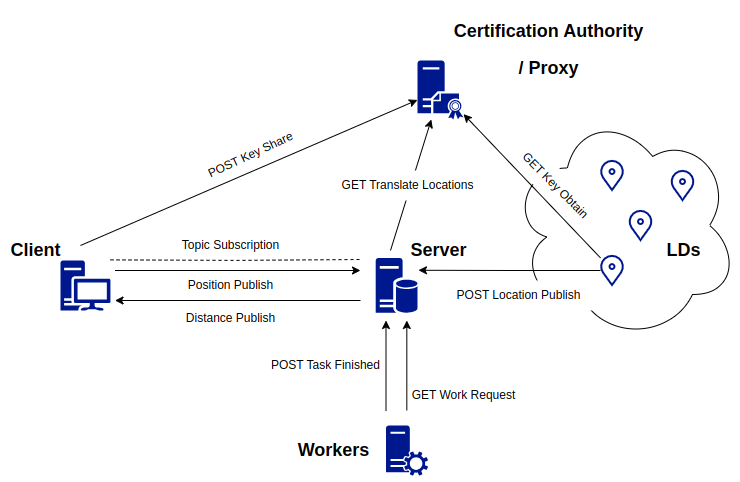
\includegraphics[width=12cm,height=7.5cm]{img/workflow.png}
    \caption{Visualization of the protocol flow}
    \label{fig:protocol-flow}
\end{figure}

\subsection{Protocol Flow}

We can summarize the protocol flow in the following steps as shown in \cref{fig:protocol-flow}:

\begin{enumerate}
    \item The clients and the parking spots register to the system, after that they receive the general position encoding parameter from the server using the \textbf{Position Encoding Parameters} API via HTTP GET request. The parameters are used to encode the positions of the clients and the parking spots. \emph{(API: \texttt{Position Encoding Parameters}, Payload: \{none\} $\to \{encoding\_params: [\text{z-order}, \text{precision}, \text{working area}, \text{grid cell size}]\}$})
    \item The mobile client $MC_i$ generates a new public/private key pair $(k_{mc_i}^+, k_{mc_i}^-)$ and sends the public key to the certification authority (CA) using the \textbf{Key Share} API via an HTTP POST request. \emph{(API: \texttt{Key Share}, Payload: $\{id: ID_{mc_i},\ k_{mc_i}^+\} \to { \text{None} }$)}
    \item After the CA verifies the client, it generates a symmetric key $k_{mc_i, park_j}$ for each parking spot $park_j$. The operation of key generation is performed by \emph{Key Translation}$(pp, k_{mc_i}^+, k_{park_j}^-)$, where $pp$ is the public parameters of the system, $k_{mc_i}^+$ is the public key of the client, and $k_{park_j}^-$ is the private key of the parking spot. Note that the translation operation must be done each time a new parking spot is added to the system.
    \item The $MC_i$ establish a MQTT connection with the server and subscribes to the topic $ID_{MC_i}$, which is used to receive updates on the parking spots. This is done using the \textbf{Topic Subscription} API via MQTT. \emph{(API: \texttt{Topic Subscription}, Payload: $\{topics: [position, distance]\}$)}
    \item The client will then send the encrypted position $\xi_{mc}(P_i)$ to the server, where $P_i$ is the encoded position of the client. The encryption is done using the public key $k_{mc_i}^+$, ensuring that only the client can decrypt the position. This is done using the \textbf{Position Publish} API via MQTT. \emph{(API: \texttt{Position Publish}, Payload: $\{position: \xi_{mc}(P_i)\}$)}
    \item The server receives the location and start the translation process, by invoking the \textbf{Translate Locations} API via HTTP GET request to the CA. The CA then re-encrypts the position for each parking spot using the associated key $k_{park_j \to mc_i}$, creating the re-encrypted blob $[\forall j \in \text{P},\ \xi_{mc_i}(P_j)]$. \emph{(API: \texttt{Translate Locations}, Payload: $\{positions: [\xi_{park_j}(P_j)]\}$)}
    \item The server will then spread the re-encrypted positions to the workers, by invoking the \textbf{Work Request} API via HTTP GET request. The workers will then compute the distances between the client position and the parking spots, using the re-encrypted positions. \emph{(API: \texttt{Work Request}, $Payload: \{ worker: w_i \} \to \{task: t_j \} $})
    \item Once the workers compute the distances (or other metrics) between client and parking spots, they send the result back using the \textbf{Task Finished} API via HTTP POST request. The result is a re-encrypted blob containing the distances between the client position and the parking spots. \emph{(API: \texttt{Task Finished}, Payload: $\{worker: w_i,\ task: t_j,\ result: \xi_{park_j \to mc_i}(R)\}$)}
    \item The server then publishes the aggregated results to the client via MQTT using the \textbf{Distance Publish} API. The payload contains the distances between the client position and the parking spots, re-encrypted with the client's public key. \emph{(API: \texttt{Distance Publish}, Payload: $\{distances: [\forall j \in P,\ \xi_{mc_i}(R)]\}$)}
    \item Finally, the client receives the re-encrypted results, decrypts them using its private key $k_{mc_i}^-$, checks weather the location satisfies the area matching condition.
\end{enumerate}

\section{Security Considerations}

The main goal of the study is to provide a privacy-preserving location-matching protocol, that allows clients to securely publish and query their positions without revealing sensitive information. In order to fulfill this goal, we need to ensure that the system is attack-resistant and that the privacy of the clients is preserved.

In the earlier approach \cite{genova2024helamqtt}, the position-matching protocol used Euclidean distance calculations between client locations and parking spots provided by a trusted CA. While the server could not directly access this data, the mechanism inadvertently exposed the positions of mobile clients (MCs). The vulnerability stemmed from the lack of client authentication, enabling malicious actors to impersonate legitimate clients and intercept traffic. An attacker could exploit this by conducting a binary search on the client’s location, sending iterative queries based on subscribed topics. By progressively refining the search area, the attacker could pinpoint the client’s exact position, violating location privacy.

This showcased that HE is secure if and only if the encryption and decryption operation are performed correctly, preferably by the client itself.

As we also mentioned in the previous attack, the system is vulnerable to a lack of authentication of the clients. Moreover, if an attacker was able to read the network traffic, he could also manipulate the communication in order to interfere with the pub/sub mechanism.

In my own implementation, I addressed those issues by introducing different techniques from the state of the art, such as using a proxy re-encryptor and a position encoding mechanism based on Z-order. The choice of leaving the decryption operation to the client ensures that no one is able to read the sensitive data, despite an increase of computational resources required to re-encrypt each position for each parking spot.

\subsection{Threat Model} \label{subsec:threatmodel}

In this section, we will analyze the threat model of the system, identifying the potential attackers and their capabilities. 


\subsection{Mitigation Strategies Malicious Actors}

\begin{table}[h]
\renewcommand{\arraystretch}{1.3}
\small
\begin{tabularx}{\linewidth}{|l|X|X|}
\hline
\textbf{Adversary} & \textbf{Goal / Attack} & \textbf{Mitigation Strategy} \\ \hline

Malicious Client &
Impersonate another client or send fake position updates. &
Use digital signatures: at the time of authentication with the CA the client signs a digital contract that ensures that he is the one trying to access the system. \\ \hline

Malicious Worker &
Manipulate computation results or leak client-sensitive data. &
Because the user has no way of finding out if an information has been manipulated during homomorphic phase, the server need to implement a mechanism of \emph{fake workload} to test workers reliability. \\ \hline

Malicious Server &
Access or manipulate sensitive client data or computational outcomes. &
Because the server could only drop the communication or modify packets, but not leak sensitive informations. It's suggested to have multiple backup servers independent one from the other. \\ \hline

Network Attacker &
Intercept and read client-sensitive data from network traffic. &
All the traffic is HE encrypted. \\ \hline

\end{tabularx}
\caption{Adversarial Threats and Mitigation Strategies}
\label{table:adversaries}
\end{table}

In the \cref{table:adversaries}, we summarize the potential adversaries and their goals, along with the mitigation strategies that can be employed to counteract their attacks. It's also important to notice that one of the assumptions of the system was that the CA is a trusted entity, moreover if an attacker is able to compromise the CA, he can also compromise the whole system. Thus, it's not worth to consider the CA as an adversary.


\chapter{Testing}
\section{Testing Methodology}

For the testing of the protocol, we implemented a proof-of-concept in Python, using the OpenFHE library\cite{openFHE}. The testing methodology consists of the following steps: firstly, we generate a set of random positions for the parking spots. After that we generated a random position for the client, we computed the z-order encoding for both the client and the parking spots, and finally we computed the distances between the client position and the parking spots using the homomorphic encryption scheme.

\section{Performance Evaluation}

What tested:
\begin{itemize}
    \item Encryption and decryption time for the client position
    \item Distance computation time for the workers
    \item Overall time for the protocol execution
    \item Comparison with clear computation for the client
\end{itemize}

\begin{figure}[h]
    \centering
    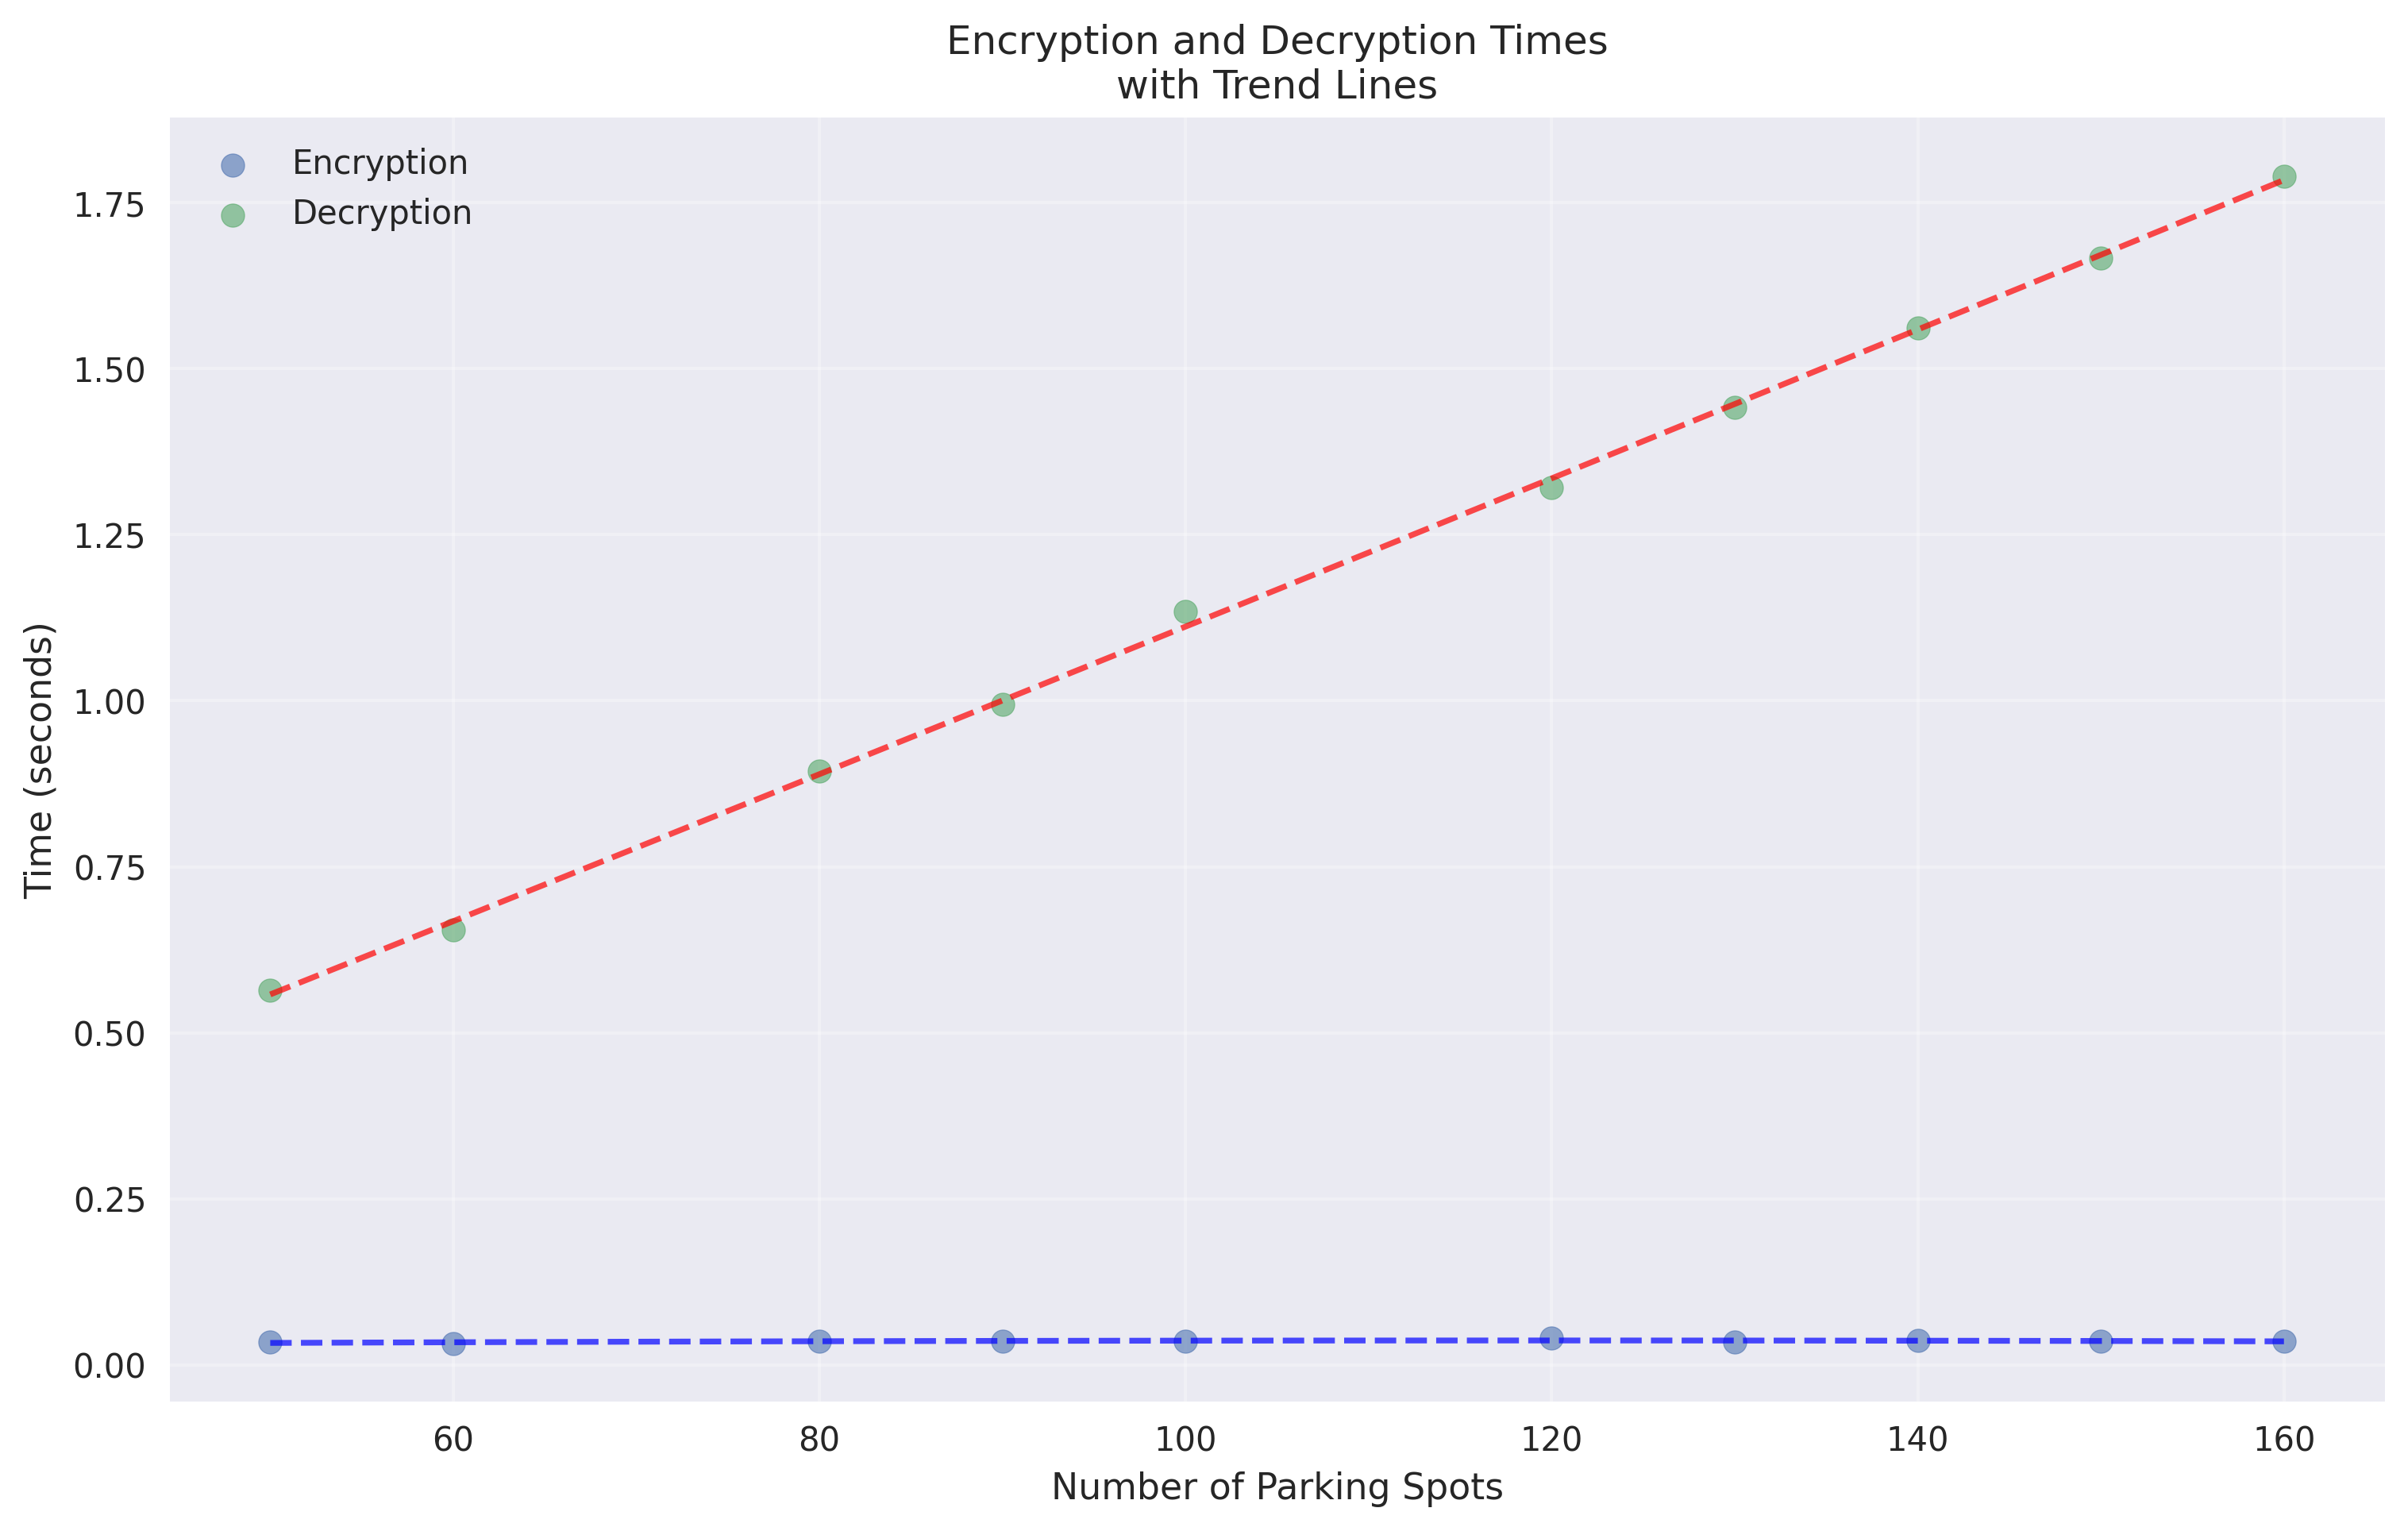
\includegraphics[width=8.5cm,height=7cm]{img/crypto_times.png}
    \caption{Visualization of the Encryption and Decryption time using HE}
    \label{fig:testing}
\end{figure}

\begin{figure}[h]
    \centering
    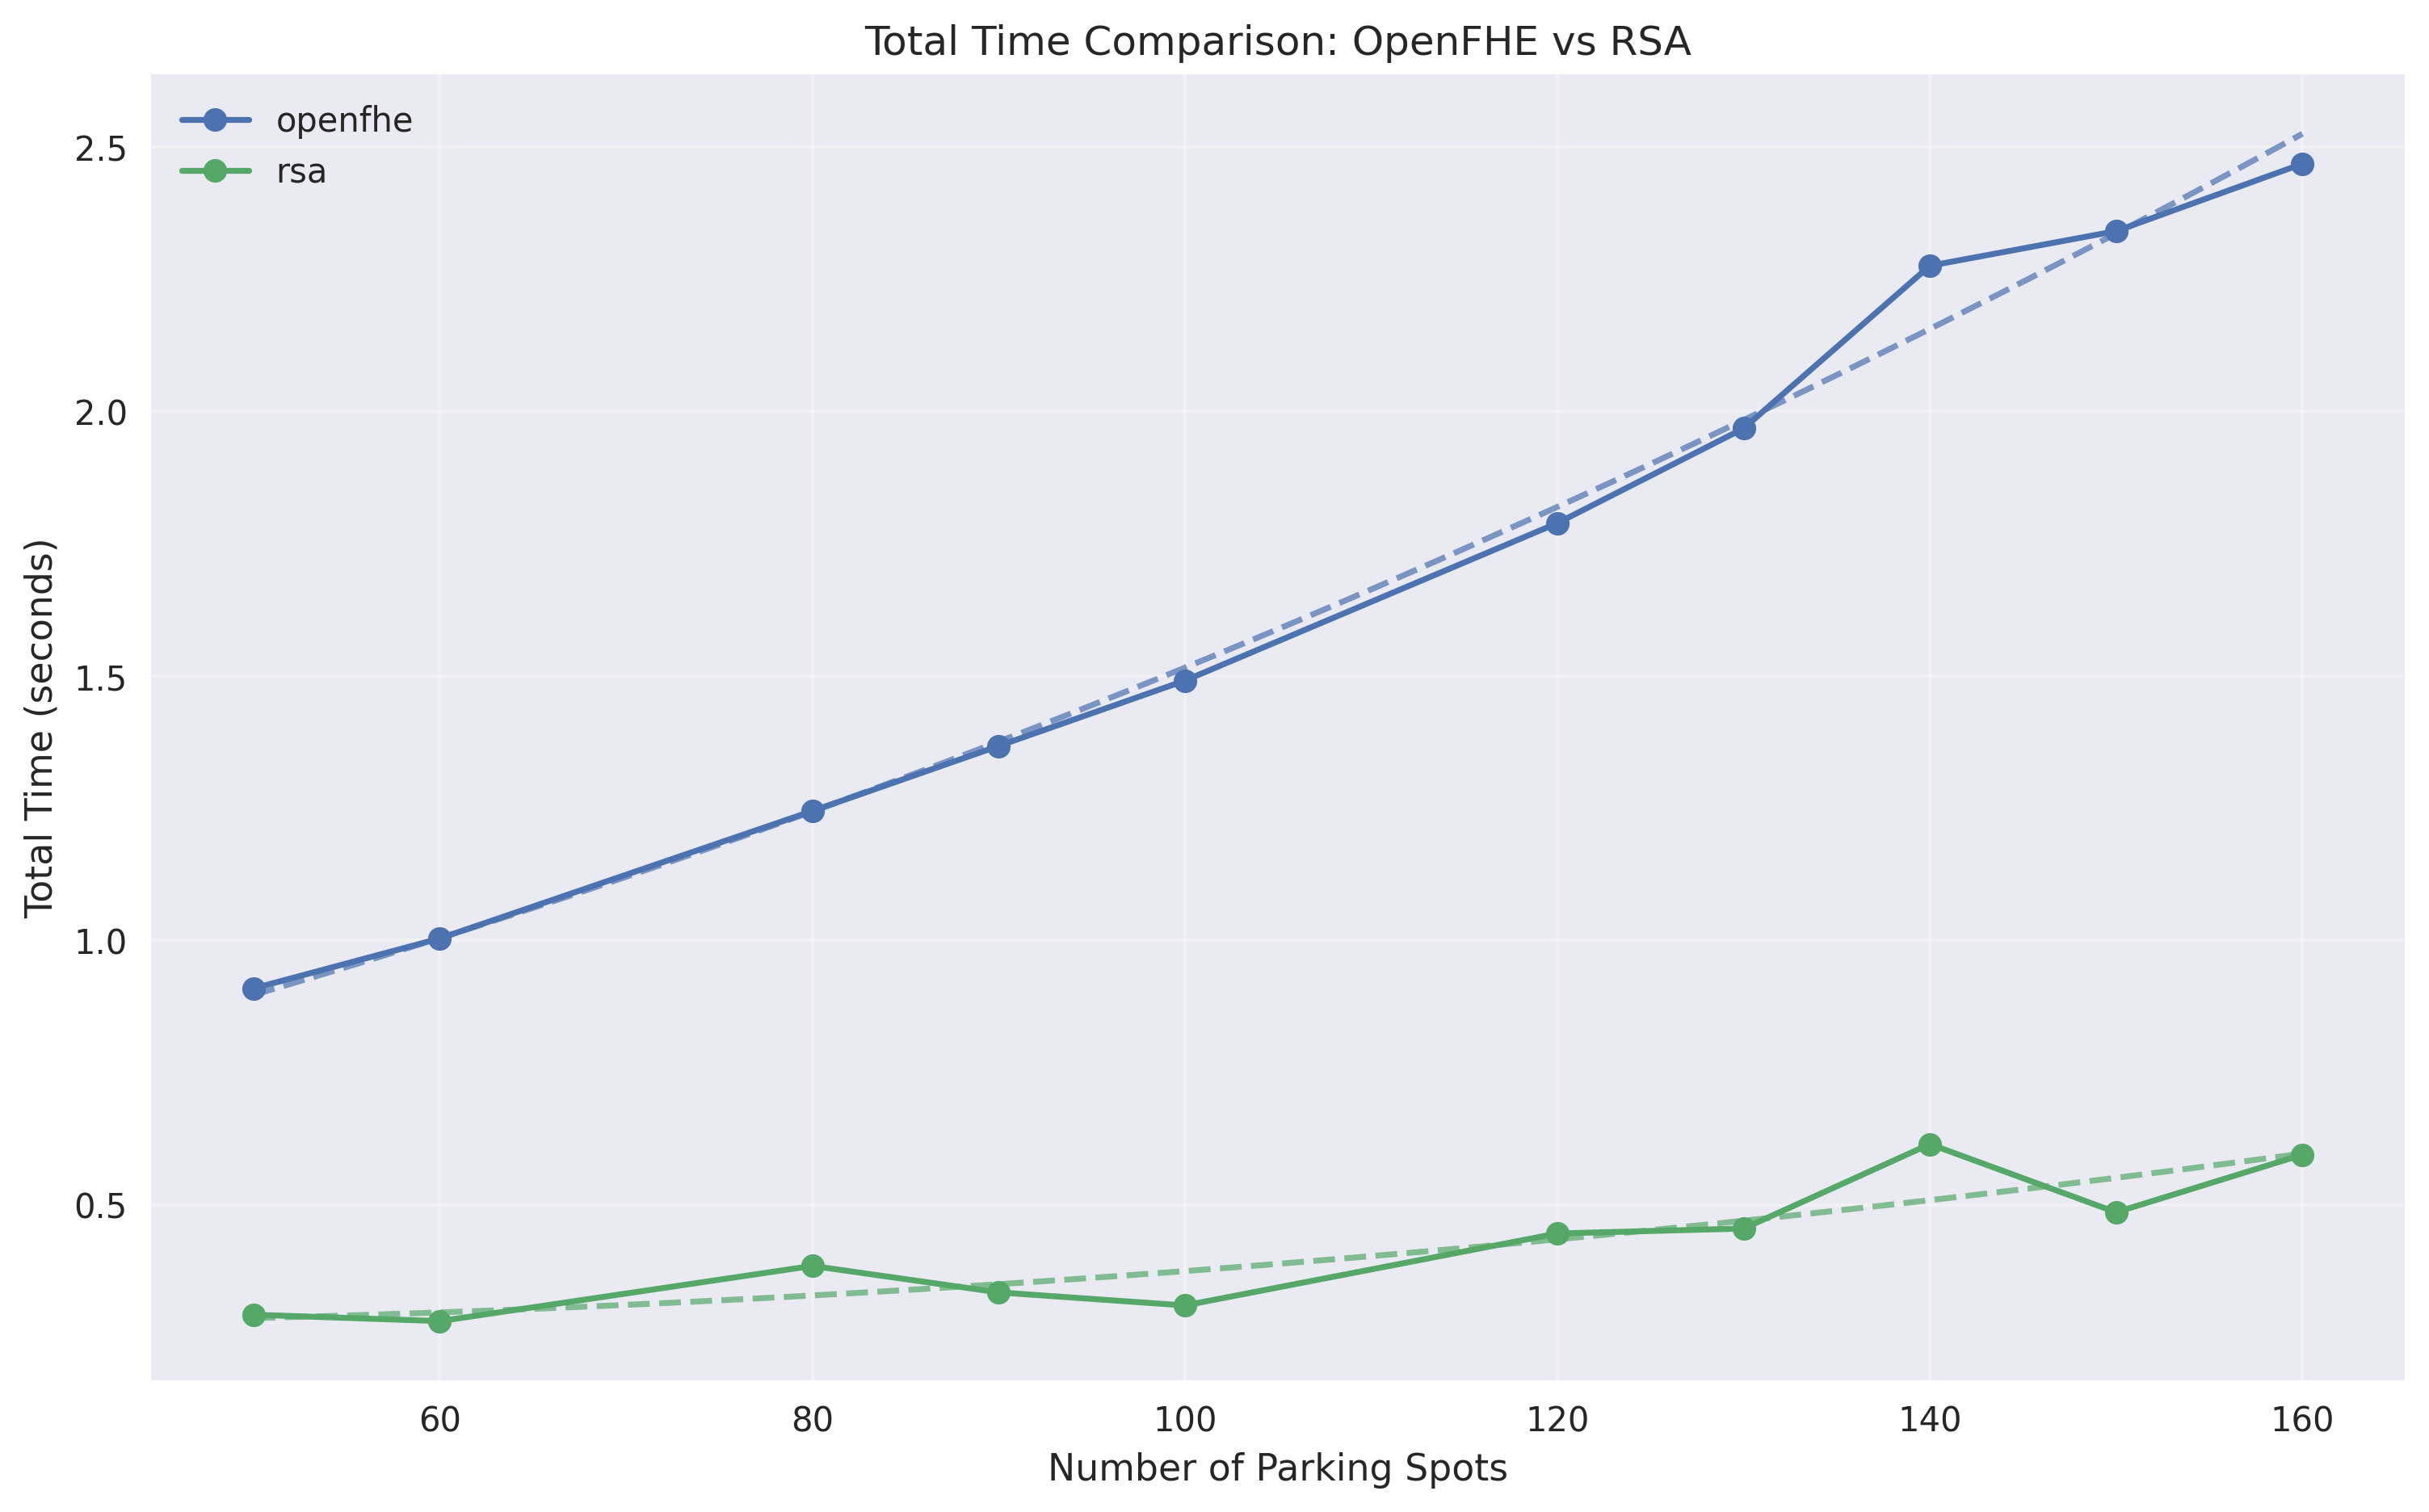
\includegraphics[width=8.5cm,height=7cm]{img/total_time_comparison.png}
    \caption{Comparison between RSA and HE for encryption and decryption}
    \label{fig:he-vs-rsa}
\end{figure}

\section{Security Analysis}

\section{Future Work}
\begin{itemize}
    \item Integrazione della libreria \emph{SEAL Embedded} per i sensori
    \item Definizione della funzione per il calcolo delle distanze
    \item Analisi degli ordini di grandezza degli errori
    \item Selezione delle posizioni rilevanti:
    \begin{itemize}
        \item Area poligonale (due punti)
        \item Area discreta (MGRS)
    \end{itemize}
    \item Deduplicazione di vettori numerici
    \item Ottimizzazione delle richieste per evitare attacchi DoS
    \begin{itemize}
        \item Dimostrazione delle vulnerabilità nell'implementazione precedente
        \item Proposta di patch risolutive
    \end{itemize}
\end{itemize}


\section{Conclusion}

\begin{itemize}
    \item Il test di fattibilità ha dimostrato che l'implementazione del protocollo è possibile e funzionale.
    \item I tempi di esecuzione sono accettabili per un utilizzo in scenari reali.
    \item la sicurezza del protocollo è garantita sotto il threat model considerato
    \item rimane comunque computaziononalmente piu' costoso rispetto ad una soluzione RSA, ma puo' essere applicato ad uno scenario zero trust.
    \item il protocollo è scalabile orizzontalmente in quanto server e sensori ma la CA no.
\end{itemize}



\renewcommand{\bibsection}{}
\chapter*{References}
\bibliography{refs}
\newpage

\renewcommand{\appendixtocname}{Appendices}
% \csname @openrightfalse\endcsname
\pagenumbering{gobble}

\newpage~\newpage
\chapter*{Ringraziamenti}
Grazie a tutti
\end{document}
